\documentclass{beamer}
\usepackage[english]{layout}
\usepackage[utf8]{inputenc}
\usepackage[english]{babel}
\usepackage[T1]{fontenc}
\usepackage{lmodern}
\usepackage{textcomp}
\usepackage{amsmath, soul, color, multicol, type1cm, verbatim, latexsym, dsfont, float, listings,alltt}
\usepackage[official]{eurosym}
\usepackage{beamerthemesplit}
\usetheme{Frankfurt}
\usefonttheme{professionalfonts}
\setbeamercovered{transparent}
%NeSI Colors <-------------------------------------------------------------------------------------
\usecolortheme{lily}
\usecolortheme[RGB={47, 68, 71}]{structure} 
\definecolor{nesidark}{HTML}{2F4447}
\definecolor{nesilight}{HTML}{CED9DF}
\definecolor{nesigrey}{gray}{0.7}
\definecolor{nesilightgrey}{gray}{0.98}
\definecolor{nesidarkgrey}{gray}{0.3}
\definecolor{nesiblue}{HTML}{2B9FC2}
\setbeamercolor{block title}{fg=black,bg=nesigrey}
\setbeamercolor{block body}{bg=nesilightgrey,fg=nesidarkgrey}
\setbeamercolor{block body alerted}{bg=white,fg=black}
\setbeamercolor{alerted text}{bg=white,fg=black}
%NeSI Title <---------------------------------------------------------------------------------------
\setbeamerfont{title}{size=\huge}
\frenchspacing
\hyphenation{NeSI}
%NeSI Template parameters <-------------------------------------------------------------------------
\setbeamertemplate{blocks}[default]
\useinnertheme{circles}
\setbeamertemplate{footline}
{
 \leavevmode
 \begin{beamercolorbox}[wd=.35\paperwidth,ht=2.25ex,dp=1ex,center]{author in head/foot}
   \usebeamerfont{author in head/foot}\insertshortauthor
 \end{beamercolorbox}
 \begin{beamercolorbox}[wd=.65\paperwidth,ht=2.25ex,dp=1ex,center]{title in head/foot}
   \usebeamerfont{title in head/foot}\insertshorttitle
 \end{beamercolorbox}
 \vskip0pt
}
\setbeamertemplate{title page}[default][center,rounded=false,shadow=false]
\newcommand\BackgroundPicture[1]{%
	\setbeamertemplate{background}{%
		\parbox[c][\paperheight]{\paperwidth}{%
			\vfill \hfill \includegraphics[height=0.9\paperheight]{#1}
			\hfill \vfill
		}
	}
}

%Content Starts Here <-------------------------------------------------------------------------------
\title{Studying allosteric enzyme inhibition using simulated molecular dynamics}
%\subtitle{Computational Science team}
\author{Ben Roberts \\(ben.roberts@nesi.org.nz)}
\date{}

\begin{document}

{
\setbeamertemplate{background canvas}{
\includegraphics[height=0.99\paperheight]{NeSI_img/Slide00.png}} 
\begin{frame}[plain]
\vspace{1cm}
\titlepage
\end{frame}
}


% This will generate the outline. If you have several topics, uncomment the multicols 
\begin{frame}
\frametitle{Outline}
% \begin{multicols}{2} 
   \tableofcontents
% \end{multicols}
\end{frame}


%%%%%%%%%%%%%%%%%%%%%%%%%%%%%%%%%%%%%%%%%%%%%%%%%%%%%%%%%%%%%%%%%%%%%%%%%%%%%%%%%%%%%%%%%%%%%%%
%%%%%%%%%%%%%%%%%%%%%%%%%%%%%%%%%%%%%%%% Some Examples %%%%%%%%%%%%%%%%%%%%%%%%%%%%%%%%%%%%%%%%%%%
%%%%%%%%%%%%%%%%%%%%%%%%%%%%%%%%%%%%%%%%%%%%%%%%%%%%%%%%%%%%%%%%%%%%%%%%%%%%%%%%%%%%%%%%%%%%%%%

\section{Background}

\subsection{Antibiotic resistance}
% List with bullets (itemize) <---
% The [<+-| alert@+>] will create a new slide for each element with highlighting 
\frame[t]
{
  \frametitle{Houston, we have a problem.}
   \begin{block}{Resistance to antibiotics is growing...}
   \begin{itemize}%[<+-| alert@+>]
	\item Mid 1940s: Mass production of penicillin
	% Italic rather than emphasised
	\item Late 1940s: Penicillin-resistant \textit{Staphylococcus aureus}
	\item MRSA, gonorrhoea, etc.
	\item 70+ years of whack-a-mole...only worse.
   \end{itemize}
  \end{block}
   \begin{block}{The search for new antibiotics}
   \begin{itemize}%[<+-| alert@+>]
	\item Try to block a bacterial enzyme
	\item We look for pathways not found in animals
   \end{itemize}
  \end{block}
}

% List with bullets (itemize) <---
% The [<+-| alert@+>] will create a new slide for each element with highlighting 
\subsection{Allosteric regulation}
\frame[t]
{
  \frametitle{Enzyme Inhibition}
   \begin{block}{Competitive inhibition}
   \begin{itemize}%[<+-| alert@+>]
	\item Binding in the active site
	\item Competes with substrate for room
   \end{itemize}
   \end{block}
   \begin{block}{Uncompetitive, non-competitive, or mixed inhibition}
   \begin{itemize}%[<+-| alert@+>]
	\item Does not compete with substrate for binding, but:
	\item Reduces affinity of enzyme for substrate, catalytic activity, or both
	\item Often involves binding at another site (``allosteric inhibition'')
   \end{itemize}
\end{block}
}

% Include Graphics <---
\frame[t]
{
  \frametitle{Enzyme Inhibition}
\begin{center}
 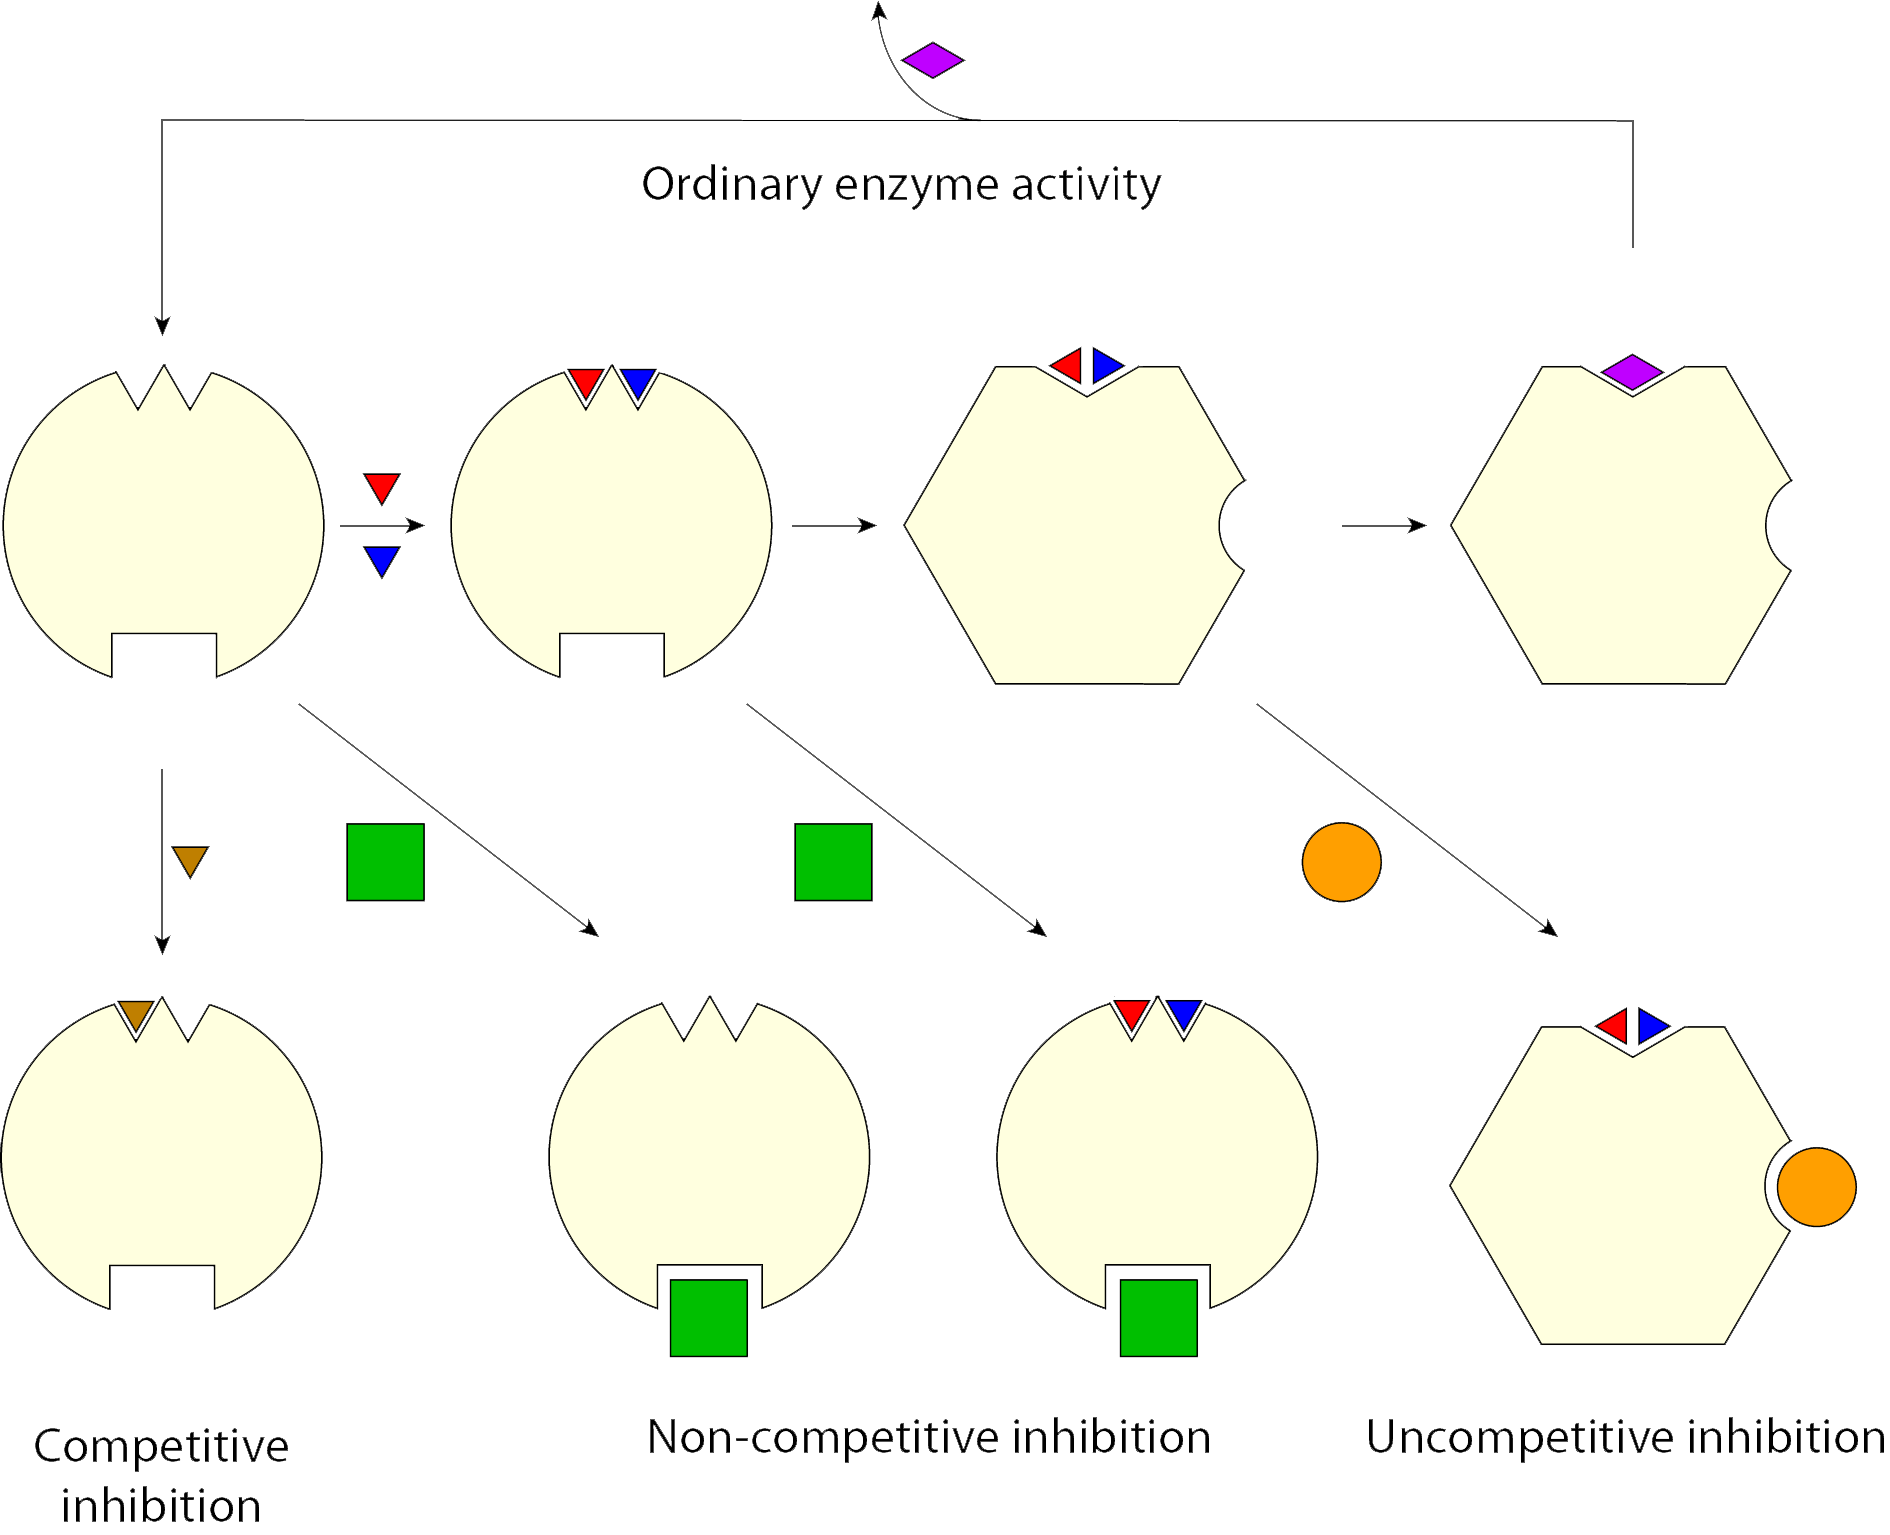
\includegraphics[width=0.75\textwidth]{Enzyme_inhibition.png}
\end{center}
}

% Include Graphics <---
\subsection{The shikimate pathway}
\frame[t]
{
  \frametitle{Aromatic Amino Acid Biosynthesis}
\begin{center}
 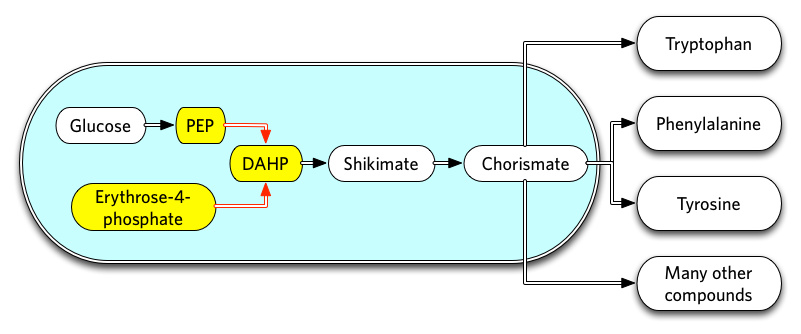
\includegraphics[width=0.9\textwidth]{bacterium_with_pathway.png}
\end{center}
 \begin{block}{The shikimate pathway}
 \begin{itemize}%[<+-| alert@+>]
	\item Bacteria, fungi, plants, etc., but not humans or animals
	\item First enzyme: DAHP synthase (step in yellow and red)
 \end{itemize}
\end{block}
}

\frame[t]
{
\frametitle{DAHP Synthase}
\begin{center}
 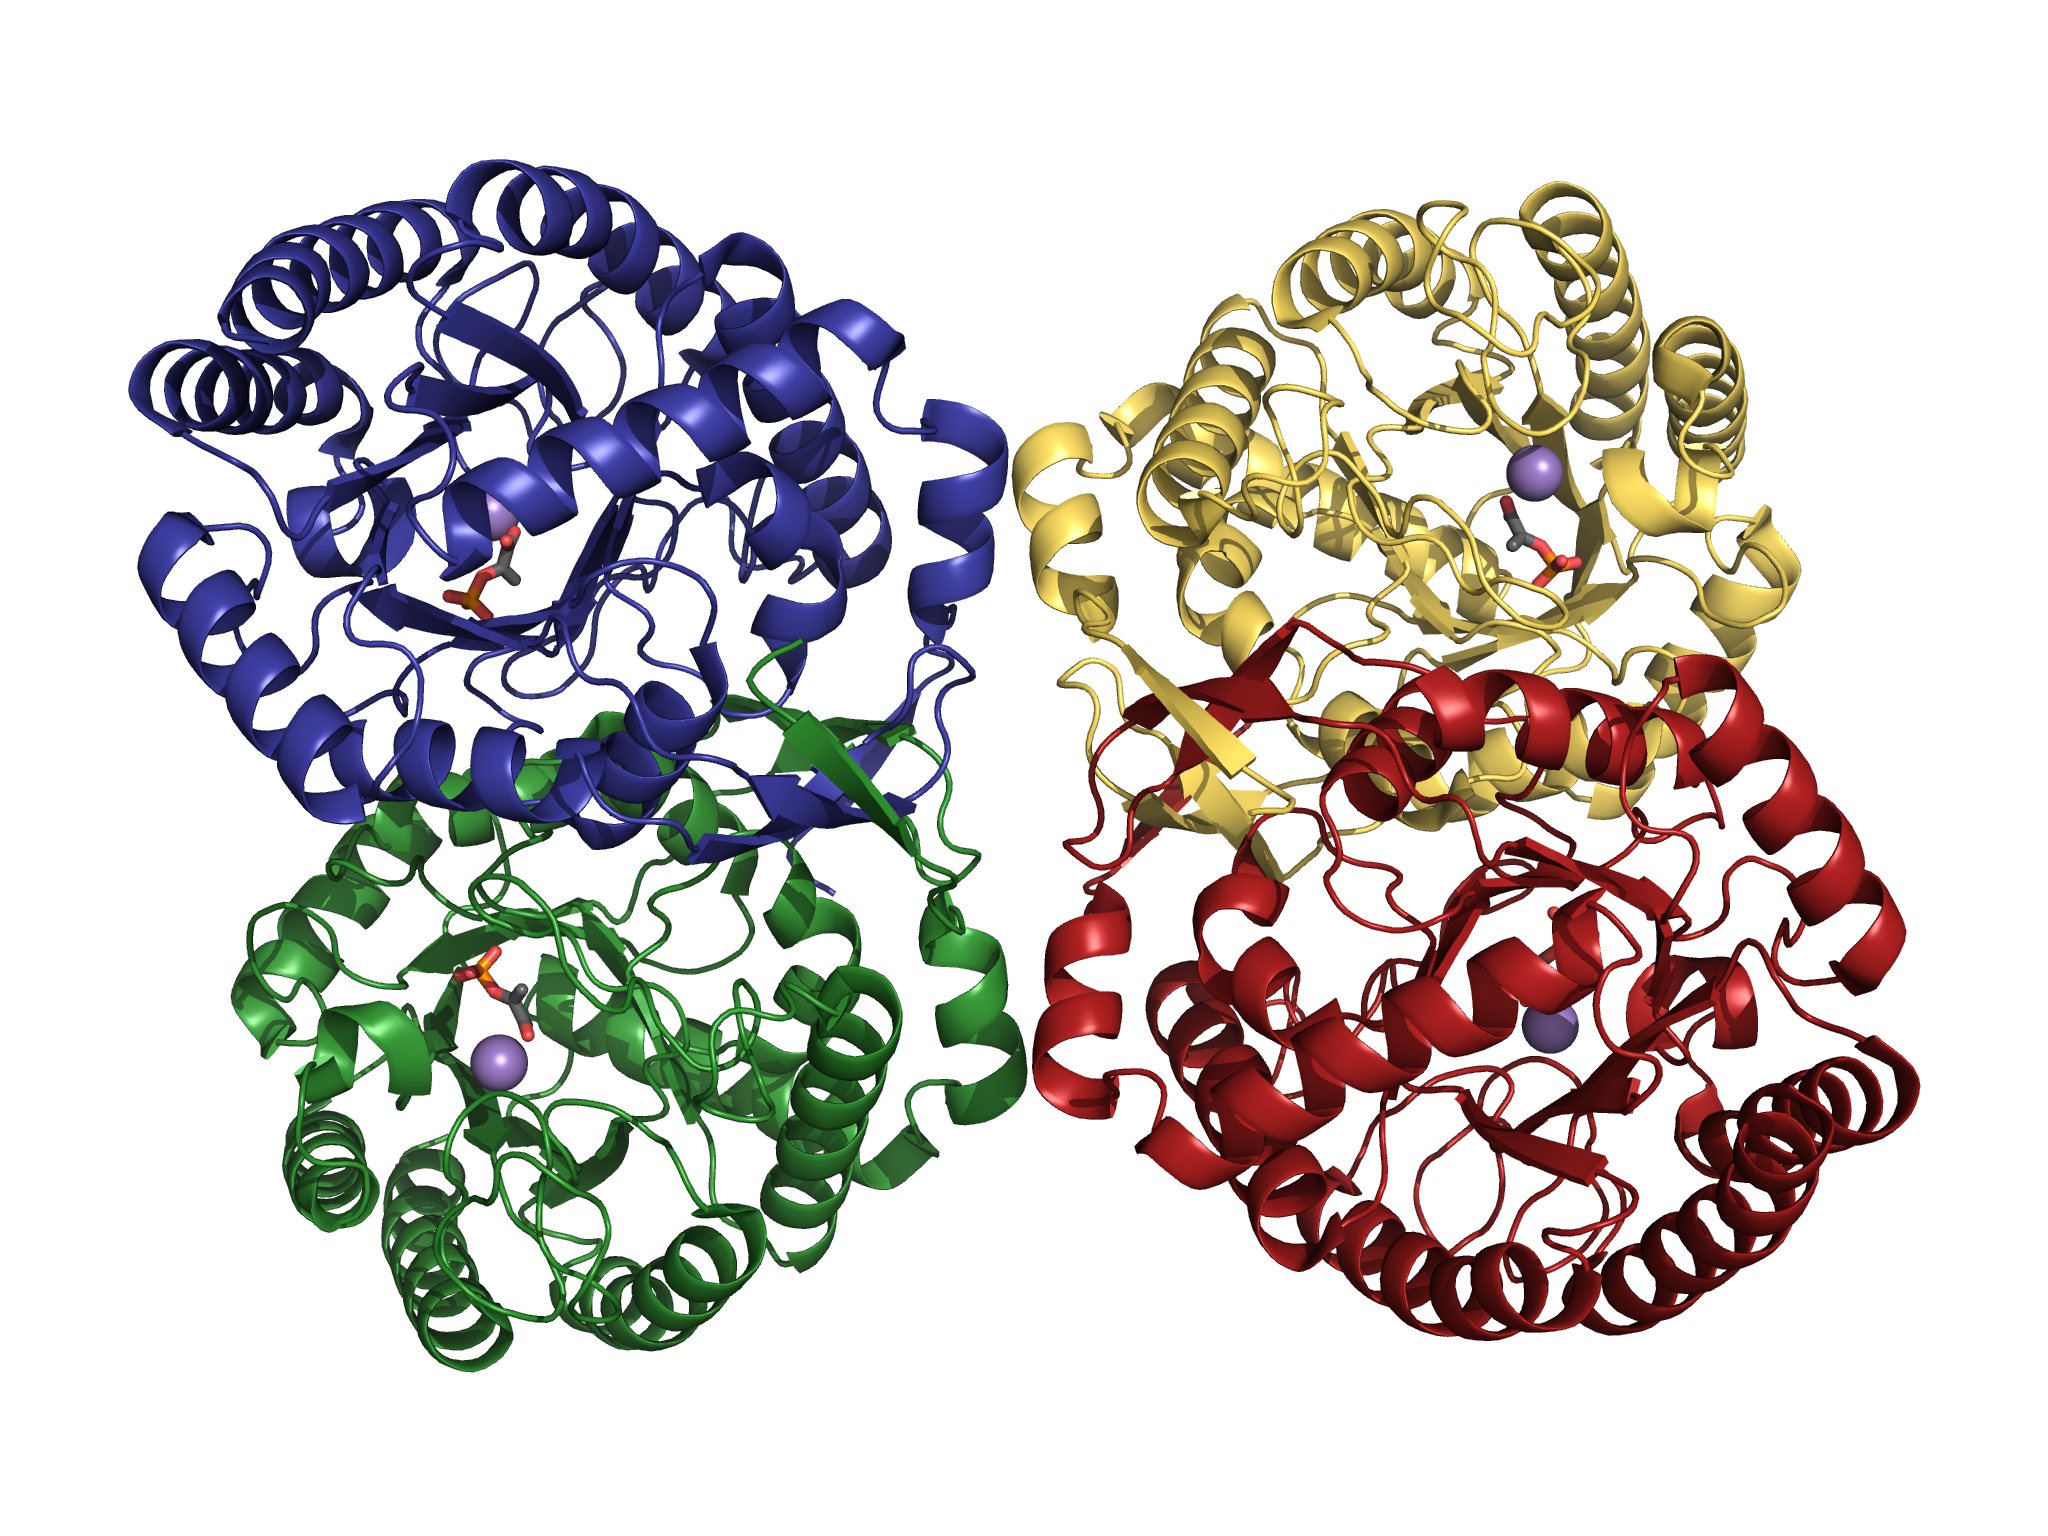
\includegraphics[width=0.9\textwidth]{4HSN_pymol.png}
\end{center}
}


\section{The Story So Far}

\subsection{MD simulations}
\frame[t]
{
  \frametitle{What can we study?}
   \begin{block}{Molecular dynamics simulations of:}
   \begin{itemize}%[<+-| alert@+>]
	\item Enzymes from different bacterial species
	\item Wild-type vs various mutants
	\item Open vs closed
	\item Presence vs absence of inhibitor
   \end{itemize}
  \end{block}
}

\frame[t]
{
\frametitle{Simulations so far:}
\begin{block}{Open vs closed (\textit{T. maritima})}
\begin{center}
 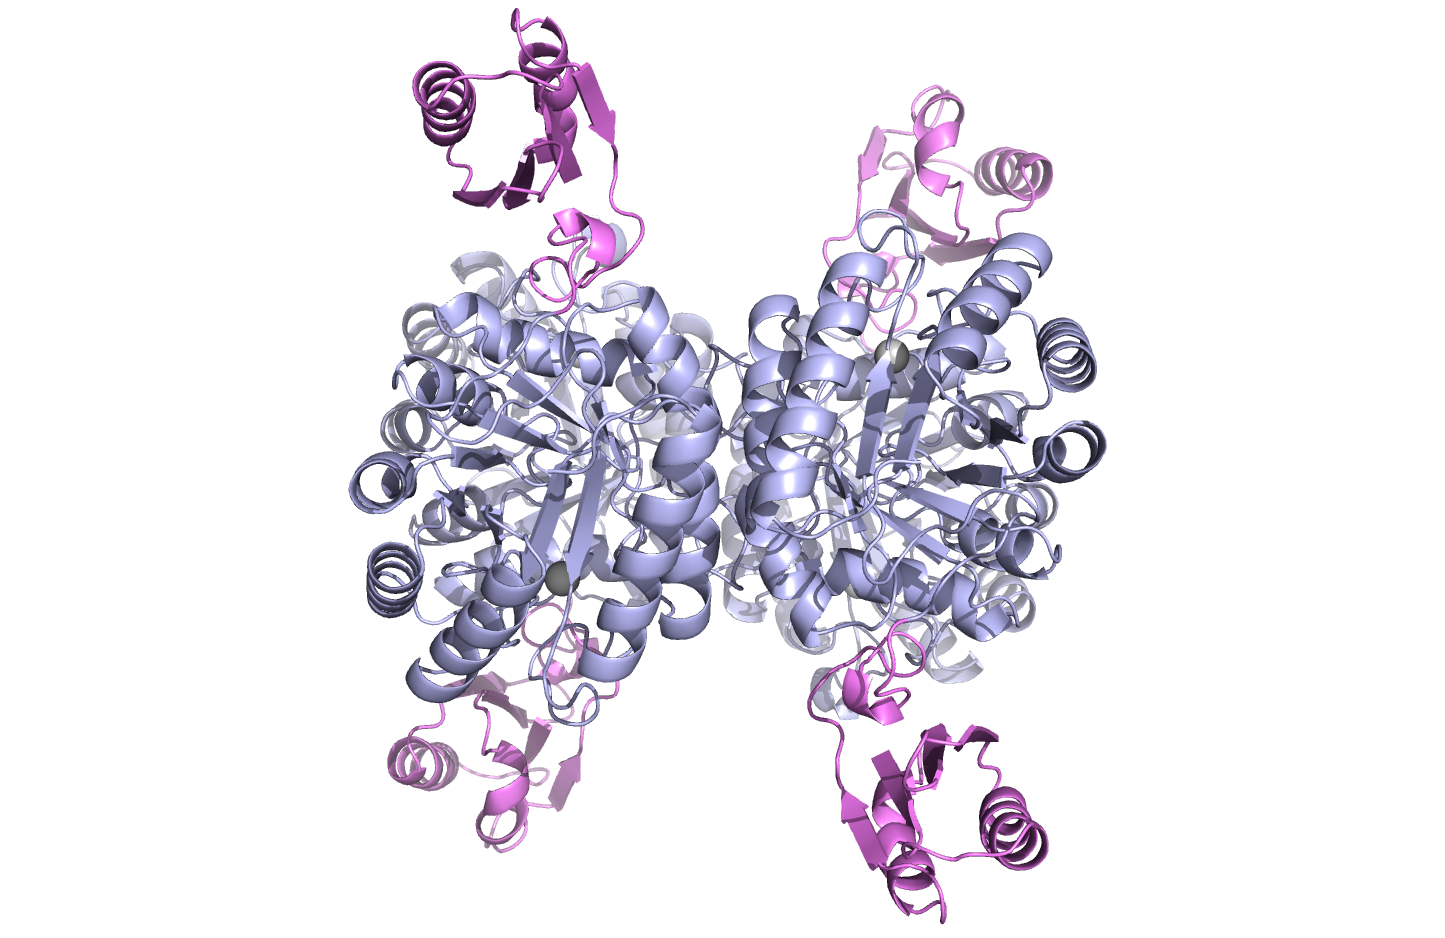
\includegraphics[width=0.4\textwidth]{T_maritima_open.png}
 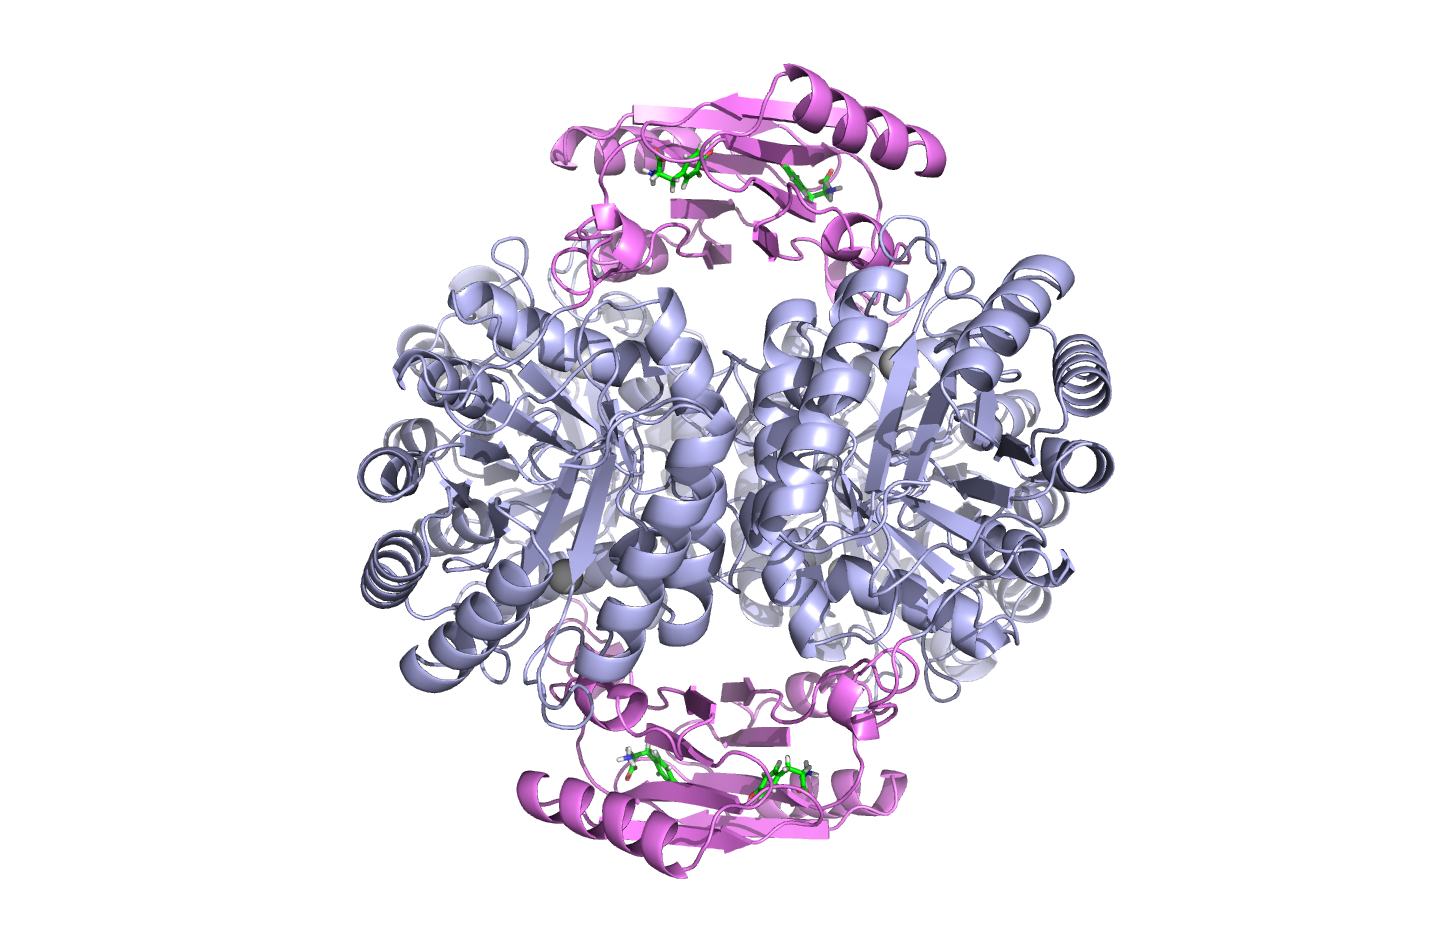
\includegraphics[width=0.4\textwidth]{T_maritima_closed.png}
\end{center}
\end{block}
\begin{block}{Presence vs absence of tyrosine}
	\begin{itemize}
		\item Conformation and dynamics
		\item Free-energy changes
	\end{itemize}
\end{block}
}

\subsection {NeSI's role}
\frame[t]
{
  \frametitle{How NeSI has helped}
   \begin{block}{Computers}
   \begin{enumerate}%[<+-| alert@+>]
	\item Computing power on BlueGene/P and POWER 7
	\item Software: NAMD (simulations), Amber (post-processing)
   \end{enumerate}
  \end{block}
   \begin{block}{Expertise}
   \begin{enumerate}%[<+-| alert@+>]
	\item Installing and configuring Amber
	\item Expert MD advice
	\item Avoiding the ``waste-of-life'' file
   \end{enumerate}
  \end{block}
}

\section{Wrap-Up}
\begin{frame}
	\frametitle{To Summarise...}
	\begin{itemize}
		\item Hundreds of ns of time simulated
		\item Amber has been deployed on POWER 7
		\item Closed form is stable when simulated
		\item Open form is extremely dynamic
		\item Does tyrosine cause closure; if so, how?
		\item Next step: Free energy calculations
	\end{itemize}
\end{frame}

\section{Acknowledgements}
\begin{frame}
  \frametitle{Acknowledgements}
   \begin{itemize}
	\item Eric Lang
	\item Emily Parker
	\item Fran\c{c}ois Bissey
	\end{itemize}
\end{frame}


% End <-----------------------------------------------------------------------------------------
{
  \setbeamertemplate{background canvas}{
\includegraphics[height=0.99\paperheight]{NeSI_img/Slide00.png}} 
  \begin{frame}[plain]
    \begin{center}
    {\Huge Questions \& Answers}
    \end{center}
  \end{frame}
}


\end{document} 
